\documentclass[border=8pt]{standalone}
\usepackage{amsmath,amssymb}
\usepackage{tikz}
\usetikzlibrary{arrows.meta}
\begin{document}
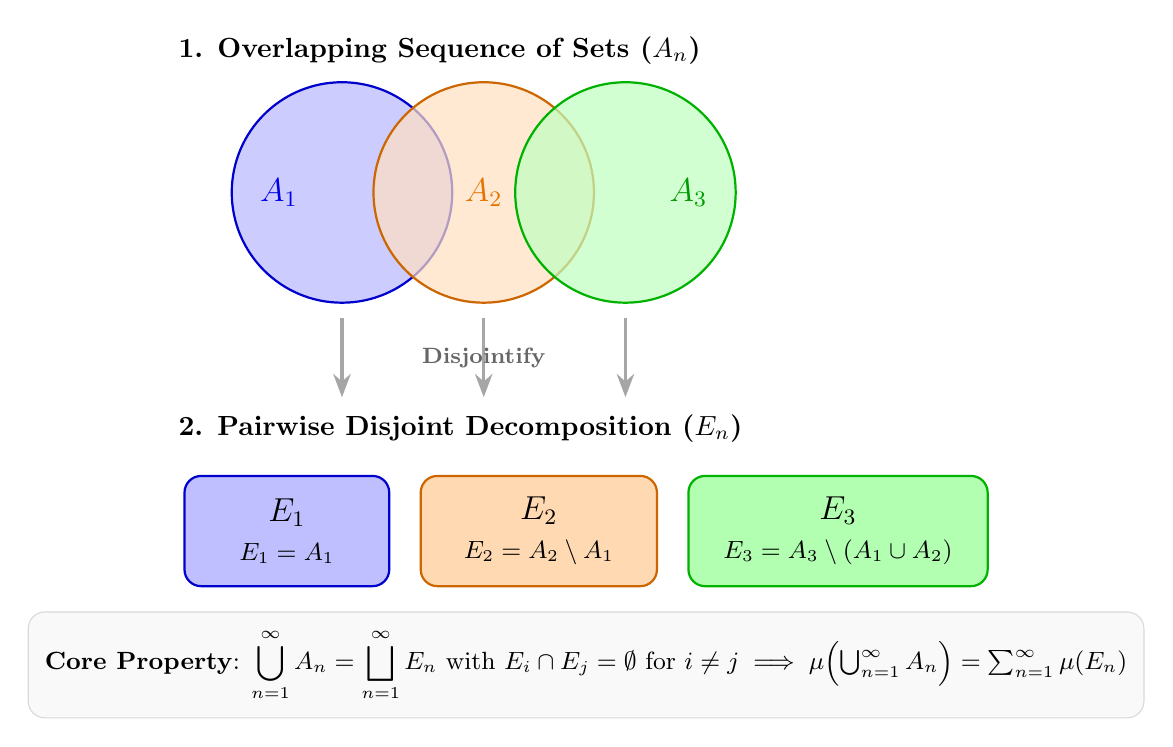
\begin{tikzpicture}[font=\small, >=Stealth]
  % Panel A: Overlapping sequence
  \node[font=\bfseries, anchor=west] at (0, 3.8) {1. Overlapping Sequence of Sets ($A_n$)};
  
  \draw[thick, fill=blue!20, draw=blue!80!black] (2.2, 2.0) circle (1.4);
  \draw[thick, fill=orange!25, fill opacity=0.7, draw=orange!80!black] (4.0, 2.0) circle (1.4);
  \draw[thick, fill=green!25, fill opacity=0.7, draw=green!70!black] (5.8, 2.0) circle (1.4);

  \node[font=\bfseries\large, blue!90!black] at (1.4, 2.0) {$A_1$};
  \node[font=\bfseries\large, orange!90!black] at (4.0, 2.0) {$A_2$};
  \node[font=\bfseries\large, green!60!black] at (6.6, 2.0) {$A_3$};

  % Downward arrows indicating disjointification
  \draw[->, very thick, gray!70] (2.2, 0.4) -- (2.2, -0.6);
  \draw[->, very thick, gray!70] (4.0, 0.4) -- (4.0, -0.6);
  \draw[->, very thick, gray!70] (5.8, 0.4) -- (5.8, -0.6);
  \node[font=\footnotesize\bfseries, text=gray!80!black] at (4.0, -0.1) {Disjointify};

  % Panel B: Disjointified pieces
  \node[font=\bfseries, anchor=west] at (0, -1.0) {2. Pairwise Disjoint Decomposition ($E_n$)};

  % Piece 1
  \draw[thick, fill=blue!25, draw=blue!80!black, rounded corners=6pt] (0.2, -3.0) rectangle (2.8, -1.6);
  \node[align=center] at (1.5, -2.3) {\textbf{\large $E_1$}\\[3pt] $E_1 = A_1$};

  % Piece 2
  \draw[thick, fill=orange!30, draw=orange!80!black, rounded corners=6pt] (3.2, -3.0) rectangle (6.2, -1.6);
  \node[align=center] at (4.7, -2.3) {\textbf{\large $E_2$}\\[3pt] $E_2 = A_2 \setminus A_1$};

  % Piece 3
  \draw[thick, fill=green!30, draw=green!70!black, rounded corners=6pt] (6.6, -3.0) rectangle (10.4, -1.6);
  \node[align=center] at (8.5, -2.3) {\textbf{\large $E_3$}\\[3pt] $E_3 = A_3 \setminus (A_1 \cup A_2)$};

  % Summary note
  \node[align=center, fill=gray!5, draw=gray!30, rounded corners=6pt, inner sep=6pt] at (5.3, -4.0)
    {\textbf{Core Property}: $\displaystyle \bigcup_{n=1}^\infty A_n = \bigsqcup_{n=1}^\infty E_n$ with $E_i \cap E_j = \emptyset$ for $i \ne j \implies \mu\Bigl(\bigcup_{n=1}^\infty A_n\Bigr) = \sum_{n=1}^\infty \mu(E_n)$};
\end{tikzpicture}
\end{document}
